\sectionthree{Homogeneous linear recurrence relations}
\begin{python0}
from solutions import *; clear() 
\end{python0}

The examples in the previous section seems to indicate
that much of the computation doesn't really depend on 
the specific recurrence relation.
So with some experience with recurrence relations, we now
move on to generalizing some of the results.

Note that I'm just showing you that many of the results
in the previous section can be generalized. 
I'm not implying that you should memorize the results.
In other words the point is to show you that the
method of generating functions is powerful and can be applied to 
many cases.
When solving recurrences, I expect \textit{you} to \textit{derive} a rational
function for the generating function and then rewrite it as a power series
and collect the general coefficient.

OK. Now let's take a look at the general linear homogeneous 
recurrence relations on sequences.
Suppose $a_n$ is a linear homogeneous recurrence relation of degree $d$:
\[
a_n = c_1 a_{n-1} + \cdots + c_d a_{n-d}
\]
for $n \geq d $.
Of course we proceed as before:
Let 
\[
a(x) = \sum_{n=0}^\infty a_n x^n
\]
Hence
\begin{align*}
a(x) 
&= a_0 + a_1 x + \cdots + a_{d-1} x^{d-1} + \sum_{n=d}^\infty a_n x^n \\
&= a_0 + a_1 x + \cdots + a_{d-1} x^{d-1} 
+ \sum_{n=d}^\infty 
\bigl( 
c_1 a_{n-1} + \cdots + c_d a_{n-d}
\bigr) x^n \\
&=
 a_0 + a_1 x + \cdots + a_{d-1} x^{d-1}
 + \sum_{n=d}^\infty  c_1 a_{n-1}x^n  
+ \cdots 
+ \sum_{n=d}^\infty  c_d a_{n-d}x^n  \\
&=
 a_0 + a_1 x + \cdots + a_{d-1} x^{d-1}
 + c_1 x \sum_{n=d}^\infty  a_{n-1}x^{n-1}    
+ \cdots 
+ c_d x^d \sum_{n=d}^\infty  a_{n-d}x^{n-d}  \\
&=
 a_0 + a_1 x + \cdots + a_{d-1} x^{d-1}
+ c_1 x \sum_{n=d-1}^\infty  a_n x^n   
+ \cdots 
+ c_d x^d \sum_{n=0}^\infty  a_n x^n  \\
&= a_0 + a_1 x + \cdots + a_{d-1} x^{d-1} \\ 
&\hskip 0.5cm + c_1 x \biggl( -a_0 - a_1x - \cdots - a_{d-2}x^{d-2} + a_0 + a_1x + \cdots
a_{d-2}x^{d-2} + \sum_{n=d-1}^\infty  a_n x^n \biggr) \\
&\hskip 0.5cm + c_2 x^2 \biggl( -a_0 - a_1x - \cdots - a_{d-3}x^{d-3} + a_0 + a_1x + \cdots
a_{d-2}x^{d-3} + \sum_{n=d-2}^\infty  a_n x^n \biggr) \\
&\hskip 0.5cm + \cdots \\
&\hskip 0.5cm + c_d x^d a(x)  \\
%
&= a_0 + a_1 x + \cdots + a_{d-1} x^{d-1}  \\
&\hskip 0.5cm 
+ c_1 x \bigl( -a_0 - a_1x - \cdots - a_{d-2}x^{d-2} \bigr) + c_1x a(x)\\
&\hskip 0.5cm 
+ c_2 x^2 \bigl( -a_0 - a_1x - \cdots - a_{d-3}x^{d-3} \bigr) + c_2x^2a(x) \\
&\hskip 0.5cm + \cdots \\
&\hskip 0.5cm + c_d x^d a(x)  \\
%
&= 
a_0 + 
(a_1 - c_1a_0)x + 
(a_2 - c_1a_1 - c_2a_0) x^2 + 
(a_3 - c_1a_2 - c_2a_1 - c_3 a_0) x^3 \\ 
&\hskip 0.5cm + \cdots +
(a_{d-1} - c_1 a_{d-2} - c_2 a_{d-3} - \cdots - c_da_0)x^{d-1}  
\\
&\hskip 0.5cm + (c_1x + c_2x^2 + \cdots + c_d x^d) a(x)
\end{align*}
Hence
\[
a(x) = 
\frac
{
a_0 + (a_1 - c_1a_0)x + \cdots 
+ (a_{d-1} - c_1 a_{d-2} - c_2 a_{d-3} - \cdots - c_da_0)x^{d-1}  
}
{
1 - (c_1x + c_2x^2 + \cdots + c_d x^d)
}
\]
Not too bad.
Tedious ... but not theoretically deep.
You just have to be careful.

The case of $d = 1$ (degree 1 recurrence relation) is
\[
a(x) = 
\frac
{a_0}
{1 - c_1x}
\]
Of course I can now immediate solve the general case for $d = 1$:
\begin{align*}
a(x) 
&= \frac{a_0}{1 - c_1x} \\
&= \sum_{n=0}^\infty a_0c_1^n x^n
\end{align*}
i.e. ...

\begin{thm}
If 
\[
a_n = c_1a_{n-1} \text{ for } n \geq 1
\]
then
\[
a_n = a_0 c_1^n \text{ for } n \geq 0
\]
\end{thm}



\newpage
\begin{ex}
Let 
\begin{align*}
a_n = 
\begin{cases}
42 & \text{ if } n = 0 \\
3a_{n-1} & \text{ if } n > 0
\end{cases}
\end{align*}
Find a closed form for $a_n$ using the above theorem.
Next, derive the closed form without using the theorem.
\end{ex}


\newpage
That was easy ...
and we've solve every single linear recurrence relation of degree 1!
Note further that solving the general homogeneous case of degree 1 
is not really 
any more difficult
than solving a specific homogeneous case of degree 1 case.

Onward! ... on to $d = 2$. If
\[
a_n = c_1 a_{n-1} + c_2 a_{n-2}
\]
for $n \geq 2$, then
\begin{align*}
a(x) 
= 
\frac
{a_0 + (a_1 - c_1 a_0) x}
{1 - (c_1 x + c_2 x^2)}
\end{align*}

Of course in order to move forward, we have to factorize
\[
1 - (c_1 x + c_2 x^2)
\]
in order to apply the theory of partial fractions.
(What else can you do anyway?)
\begin{align*}
1 - (c_1 x + c_2 x^2)
= 1 - c_1 x - c_2 x^2
= -c_2 \biggl( x^2 + \frac{c_1}{c_2} x - \frac{1}{c_2} \biggr)
\end{align*}
The roots of
\[
x^2 + \frac{c_1}{c_2} x - \frac{1}{c_2}
\]
are
\[
x = 
\frac
{-\frac{c_1}{c_2} 
\pm 
\sqrt{
\bigl( \frac{c_1}{c_2} \bigr)^2
+ 4 \frac{1}{c_2}
}
}
{2}
=
\frac{-c_1 \pm \sqrt{c_1^2 + 4c_2}}{2c_2}
\]
Note that 
It's possible to have complex roots (i.e. $c_1^2 + 4c_2 < 0$)
and it's possible to have repeated roots (i.e. $c_1^2 + 4c_2 = 0$).

Let's consider the case $c_1^2 + 4c_2 = 0$ first.
Of course in this case the roots are both
\[
-\frac{c_1}{2c_2}
\]
\begin{align*}
1 - (c_1 x + c_2 x^2)
&= -c_2 \biggl( x^2 + \frac{c_1}{c_2} x - \frac{1}{c_2} \biggr) \\
&= -c_2 \biggl( x - \frac{c_1}{2c_2} \biggr)^2
\end{align*}
Therefore our generating function becomes
\begin{align*}
a(x) 
&=
\frac
{a_0 + (a_1 - c_1 a_0) x}
{1 - (c_1 x + c_2 x^2)} \\
&=
\frac
{a_0 + (a_1 - c_1 a_0) x}
{-c_2 \bigl( x - \frac{c_1}{2c_2} \bigr)^2} \\
&=
\frac {a_0 + (a_1 - c_1 a_0) x} {-c_2} \cdot
\frac{1}{\bigl(\frac{c_1}{2c_2} - x \bigr)^2}
\end{align*}
At this point it's already clear that we can rewrite the rational
function very easily into a power series.
(The computation is tedious but not deep.)
We just basically need to rewrite a rational function of the
form
\[
(A + Bx) \cdot \frac{1}{(C - x)^2}
\]
as a power series and then substitute the following:
\[
A = -\frac{a_0}{c_2}, B = -\frac{a_1 - c_1 a_0}{c_2}, 
C = \frac{c_1}{2c_2}
\]

We have
\begin{align*}
(A + Bx) \cdot \frac{1}{(C - x)^2}
&= \frac{A + Bx}{C^2} \sum_{n=0}^\infty (n+1) \frac{1}{C^n} x^n \\
&= \frac{A }{C^2} \sum_{n=0}^\infty (n+1) \frac{1}{C^n} x^n 
+ \frac{B}{C^2} \sum_{n=0}^\infty (n+1) \frac{1}{C^n} x^{n+1}
\\
&= \frac{A }{C^2} \sum_{n=0}^\infty (n+1) \frac{1}{C^n} x^n 
+ \frac{B}{C^2} \sum_{n=1}^\infty n \frac{1}{C^{n-1}} x^n
\\
\end{align*}
The coefficient of $x^0$ is
\[
\frac{A}{C^2}
\]
and the coefficient of $x^n$ for $n \geq 1$ is
\[
\frac{A}{C^2}(n+1)\frac{1}{C^n} + \frac{B}{C^2} n \frac{1}{C^{n-1}}
= \frac{1}{C^{n+1}}
\biggl(
\frac{(n+1)A}{C}
+
nB 
\biggr)
\]

Now we replace $A, B, C$ with the constants from our original problem:
\[
\frac{A}{C^2} 
=
\frac{-\frac{a_0}{c_2}}{(\frac{c_1}{2c_2})^2}
=
-\frac{a_0}{c_2} \cdot \frac{4c_2^2}{c_1^2}
\]
But wait a minute:
isn't $a_0$ the coefficient of $x^0$ for $a(x) = \sum_{n=0} a_nx^n$?!?
Not to worry:
Remember that we're in the case of repeated roots and the
condition guaranteeing that is $c_1^2  + 4c_2 = 0$.
This means that $c_1^2 = -4c_2$.
Therefore
\[
\frac{A}{C^2} 
=
-\frac{a_0}{c_2} \cdot \frac{4c_2^2}{c_1^2}
= -\frac{a_0}{c_2} \cdot \frac{4c_2^2}{-4c_2}
= a_0
\]
Phew! Check that the coefficient for $x^1$ does simplify to $a_1$.

Finally compute and simplify the closed form for
$a_n$ for $n \geq 1$ 
and complete the statement of the homogeneous
degree-2 recurrence relation
when the roots of the denominator of the rational function
for $a(x)$ has repeated roots:

\begin{thm}
Let $a_n$ ($n = 0, 1, 2, \ldots$) be a sequence satisyfing the following
degree 2 recurrence relation:
\[
a_n = c_1 a_{n-1} + c_2 a_{n-2}, \,\,\,\,\, n \geq 2
\]
Furthermore assume that
\[
c_1^2 + 4c_2 = 0
\] 
Then $a_n$ ($n = 0, 1, 2, \ldots$) has the following closed form:
XXX
\end{thm}

Now let's tackle the case where $c_1^2 + 4c_2 \neq 0$,
i.e. the denominator of the rational function for $a(x)$
has two distinct roots.
Recall that following facts: Our recurrence relation is this:
\[
a_n = c_1 a_{n-1} + c_2 a_{n-2}, \,\,\,\,\, (n \geq 2)
\]
and the rational function for $a(x) = \sum_{n=0}^\infty a_n x^n$ is
\[
\frac
{a_0 + (a_1 - c_1 a_0) x}
{1 - (c_1 x + c_2 x^2)}
\]
The denominator of the rational function is
\begin{align*}
1 - (c_1 x + c_2 x^2)
&= -c_2 \biggl( x^2 + \frac{c_1}{c_2} x - \frac{1}{c_2} \biggr)
\end{align*}
The roots of
\[
x^2 + \frac{c_1}{c_2} x - \frac{1}{c_2}
\]
are
\[
x
=
\frac{-c_1 \pm \sqrt{c_1^2 + 4c_2}}{2c_2}
\]
Of course putting everything together we have this:
\begin{align*}
a(x) 
&=
\frac {a_0 + (a_1 - c_1 a_0) x} {-c_2} \cdot
\frac{1}{x^2 + \frac{c_1}{c_2} x - \frac{1}{c_2}} \\
&= (A + Bx) \frac{1}{(x-C)(x-D)}
\end{align*}
where $A$ and $B$ are as before for the case of repeated roots 
and for $C$ and $D$ are distinct roots of the
denominator of the rational function of $a(x)$:
\[
C = \frac{-c_1 - \sqrt{c_1^2 + 4c_2}}{2c_2},
D = \frac{-c_1 - \sqrt{c_1^2 + 4c_2}}{2c_2}
\]

Note that it's possible to have complex roots.
However you don't have to worry about it since the algebra will still work,
i.e. just ignore the fact that $C$ and $D$ can be complex and simply perform
the computation.
However when $C$ and $D$ are complex there are certain steps that you can take
to speed up the computations of powers.
I'll handle the degree 2 complex roots case later.

Now go ahead and rewrite 
\[
(A + Bx) \frac{1}{(x-C)(x-D)}
\] as a power series and finish this case of your theorem:

\begin{thm}
Let $a_n$ ($n = 0, 1, 2, \ldots$) be a sequence satisyfing the following
degree 2 recurrence relation:
\[
a_n = c_1 a_{n-1} + c_2 a_{n-2}, \,\,\,\,\, n \geq 2
\]
Furthermore assume that
\[
c_1^2 + 4c_2 \neq 0
\] 
Then $a_n$ ($n = 0, 1, 2, \ldots$) has the following closed form:
\vskip 2in
\end{thm}

\newpage
\subsection*{Solutions}

\newpage
\section*{Solutions}
Solution to Exercise \ref{ex:dfa0}\labeltext{}{sol:dfa0}.

\tinysidebar{\debug{exercises/{dfa0/answer.tex}}}

    Solution not provided.
    

\newpage

Solution to Exercise \ref{ex:dfa1}\labeltext{}{sol:dfa1}.

\tinysidebar{\debug{exercises/{dfa1/answer.tex}}}
  The ID computation is
  \begin{align*}
    (q_0, aba)
    &\vdash (\delta(q_0, a), ba) = (q_0, ba) \\ 
    &\vdash (\delta(q_0, b), a) = (q_1, a) \\
    &\vdash (\delta(q_1, a), \ep) = (q_0, \ep)
  \end{align*}
  $q_0$ is not an accept state. Therefore $aba$ is not accepted.


\newpage

Solution to Exercise \ref{ex:dfa4}\labeltext{}{sol:dfa4}.

\tinysidebar{\debug{exercises/{dfa4/answer.tex}}}

    Solution not provided.
    

\newpage

Solution to Exercise \ref{ex:dfa5}\labeltext{}{sol:dfa5}.

\tinysidebar{\debug{exercises/{dfa5/answer.tex}}}

    Solution not provided.
    

\newpage

Solution to Exercise \ref{ex:implementing-a-single-dfa0}\labeltext{}{sol:implementing-a-single-dfa0}.

\tinysidebar{\debug{exercises/{implementing-a-single-dfa0/answer.tex}}}

    Solution not provided.
    

\newpage

Solution to Exercise \ref{ex:nfastatediag0}\labeltext{}{sol:nfastatediag0}.

\tinysidebar{\debug{exercises/{nfastatediag0/answer.tex}}}

    Solution not provided.
    

\newpage

Solution to Exercise \ref{ex:nfastatediag1}\labeltext{}{sol:nfastatediag1}.

\tinysidebar{\debug{exercises/{nfastatediag1/answer.tex}}}

    Solution not provided.
    

\newpage

Solution to Exercise \ref{ex:nfastatediag2}\labeltext{}{sol:nfastatediag2}.

\tinysidebar{\debug{exercises/{nfastatediag2/answer.tex}}}

    Solution not provided.
    

\newpage

Solution to Exercise \ref{ex:nfastatediag3}\labeltext{}{sol:nfastatediag3}.

\tinysidebar{\debug{exercises/{nfastatediag3/answer.tex}}}

    Solution not provided.
    

\newpage

Solution to Exercise \ref{ex:nfastatediag4}\labeltext{}{sol:nfastatediag4}.

\tinysidebar{\debug{exercises/{nfastatediag4/answer.tex}}}

    Solution not provided.
    

\newpage

Solution to Exercise \ref{ex:nfastatediag5}\labeltext{}{sol:nfastatediag5}.

\tinysidebar{\debug{exercises/{nfastatediag5/answer.tex}}}

    Solution not provided.
    

\newpage

Solution to Exercise \ref{ex:nfastatediag6}\labeltext{}{sol:nfastatediag6}.

\tinysidebar{\debug{exercises/{nfastatediag6/answer.tex}}}

    Solution not provided.
    

\newpage

Solution to Exercise \ref{ex:nfastatediag7}\labeltext{}{sol:nfastatediag7}.

\tinysidebar{\debug{exercises/{nfastatediag7/answer.tex}}}

    Solution not provided.
    

\newpage

Solution to Exercise \ref{ex:nfastatediag8}\labeltext{}{sol:nfastatediag8}.

\tinysidebar{\debug{exercises/{nfastatediag8/answer.tex}}}

    Solution not provided.
    

\newpage

Solution to Exercise \ref{ex:nfastatediag9}\labeltext{}{sol:nfastatediag9}.

\tinysidebar{\debug{exercises/{nfastatediag9/answer.tex}}}

    Solution not provided.
    

\newpage

Solution to Exercise \ref{ex:nfastatediag10}\labeltext{}{sol:nfastatediag10}.

\tinysidebar{\debug{exercises/{nfastatediag10/answer.tex}}}

    Solution not provided.
    

\newpage

Solution to Exercise \ref{ex:nfastatediag11}\labeltext{}{sol:nfastatediag11}.

\tinysidebar{\debug{exercises/{nfastatediag11/answer.tex}}}

    Solution not provided.
    

\newpage

Solution to Exercise \ref{ex:nfastatediag12}\labeltext{}{sol:nfastatediag12}.

\tinysidebar{\debug{exercises/{nfastatediag12/answer.tex}}}

    Solution not provided.
    

\newpage

Solution to Exercise \ref{ex:nfastatediag13}\labeltext{}{sol:nfastatediag13}.

\tinysidebar{\debug{exercises/{nfastatediag13/answer.tex}}}

    Solution not provided.
    

\newpage

Solution to Exercise \ref{ex:nfa0}\labeltext{}{sol:nfa0}.

\tinysidebar{\debug{exercises/{nfa0/answer.tex}}}
The formal definition of this NFA is $(\Sigma, Q, q_0, \delta, F)$ where
\begin{tightlist}
\li $\Sigma = \{a,b\}$
\li $Q = \{q_0\}$
\li $\delta$ is the function
\[
\delta : Q \times \Sigma_\epsilon \rightarrow P(Q)
\]
given by
\begin{align*}
  \delta(q_0, \epsilon) &= \{\} \\
  \delta(q_0, a) &= \{\} \\
  \delta(q_0, b) &= \{\} 
\end{align*}
\end{tightlist}


\newpage

Solution to Exercise \ref{ex:nfa1}\labeltext{}{sol:nfa1}.

\tinysidebar{\debug{exercises/{nfa1/answer.tex}}}

    Solution not provided.
    

\newpage

Solution to Exercise \ref{ex:nfa2}\labeltext{}{sol:nfa2}.

\tinysidebar{\debug{exercises/{nfa2/answer.tex}}}

    Solution not provided.
    

\newpage

Solution to Exercise \ref{ex:nfa3}\labeltext{}{sol:nfa3}.

\tinysidebar{\debug{exercises/{nfa3/answer.tex}}}

    Solution not provided.
    

\newpage

Solution to Exercise \ref{ex:nfa4}\labeltext{}{sol:nfa4}.

\tinysidebar{\debug{exercises/{nfa4/answer.tex}}}

    Solution not provided.
    

\newpage

Solution to Exercise \ref{ex:nfa5}\labeltext{}{sol:nfa5}.

\tinysidebar{\debug{exercises/{nfa5/answer.tex}}}

    Solution not provided.
    

\newpage

Solution to Exercise \ref{ex:dfa-as-powerful-as-nfa0}\labeltext{}{sol:dfa-as-powerful-as-nfa0}.

\tinysidebar{\debug{exercises/{dfa-as-powerful-as-nfa0/answer.tex}}}
Here's the solution.
Let $\delta$ denote the transition function of $N$.
Note that 
\begin{align*}
  \delta(q_0, \epsilon) = \{\} \\
  \delta(q_0, a) = \{\} \\
  \delta(q_0, b) = \{\} 
\end{align*}
First of all the states are labeled as all the subsets of $\{q_0\}$.


\begin{center}
\begin{tikzpicture}[>=triangle 60,shorten >=0.5pt,node distance=2cm,auto,initial text=, double distance=2pt]
\node[state] (A) at (  0,  0) {$\{q_0\}$};
\node[state] (B) at (  3,  0) {$\{\}$};

\path[->]

;
\end{tikzpicture}
\end{center}
    


The start state is the $\epsilon$-closure of $\{q_0\}$.
However in $N$, there are no $\epsilon$--transitions out of 
$q_0$.
So the $\epsilon$-closure of $\{q_0\}$ is in fact $\{q_0\}$, i.e.
$\overline{\{q_0\}} = \{q_0\}$
The $\DFA$ is now this:


\begin{longtable}{|r||r|r|r|r|r|}
\hline 
         & $w_1$ & $w_2$ & $w_3$ & $w_4$ & $\ldots$ \\ \hline \hline 
$M_1$    &       &       &       &       &          \\ \hline 
$M_2$    &       &       &       &       &          \\ \hline 
$M_3$    &       &       &       &       &          \\ \hline 
$M_4$    &       &       &       &       &          \\ \hline 
$\ldots$ &       &       &       &       &          \\ \hline 
\end{longtable}
        


Now I will compute the $a$--transition of the state $\{q_0\}$.
Let $\delta^\DFA$ denote the transition function of the $\DFA$
that we're building.
Then
\begin{align*}
\delta( \{q_0, a\} ) 
&= \overline{ \bigcup_{q \in \{q_0\}} \delta(q, a)} \\
&= \overline{ \delta(q_0, a) } \\
&= \overline{ \emptyset } \\
&= \emptyset
\end{align*}
The (incomplete) $\DFA$ now looks like this:


\begin{longtable}{|r||r|r|r|r|r|}
\hline 
         & $w_1$ & $w_2$ & $w_3$ & $w_4$ & $\ldots$ \\ \hline \hline 
$M_1$    & 0     & 0     & 1     & 0     & ...      \\ \hline 
$M_2$    & 1     & 0     & 1     & 1     & ...      \\ \hline 
$M_3$    & 0     & 1     & 1     & 1     & ...      \\ \hline 
$M_4$    & 1     & 0     & 1     & 1     & ...      \\ \hline 
$\ldots$ &       &       &       &       &          \\ \hline 
\end{longtable}
        


Using the same reasoning we have

\begin{center}
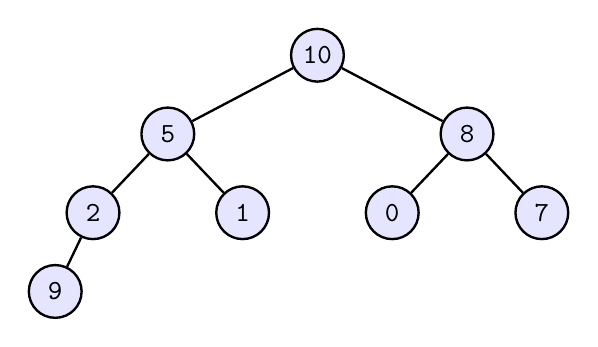
\begin{tikzpicture}

\fill[blue!10] (0.0, 0.0) circle (0.35);
\node [line width=0.03cm,black,minimum size=0.6699999999999999cm,draw,circle] at (0.0,0.0)(10){};\draw (0.0, 0.0) node[color=black] {\texttt{10}};
\fill[blue!10] (-1.9, -1.0) circle (0.35);
\node [line width=0.03cm,black,minimum size=0.6699999999999999cm,draw,circle] at (-1.9,-1.0)(5){};\draw (-1.9, -1.0) node[color=black] {\texttt{5}};
\fill[blue!10] (1.9, -1.0) circle (0.35);
\node [line width=0.03cm,black,minimum size=0.6699999999999999cm,draw,circle] at (1.9,-1.0)(8){};\draw (1.9, -1.0) node[color=black] {\texttt{8}};
\fill[blue!10] (-2.85, -2.0) circle (0.35);
\node [line width=0.03cm,black,minimum size=0.6699999999999999cm,draw,circle] at (-2.85,-2.0)(2){};\draw (-2.85, -2.0) node[color=black] {\texttt{2}};
\fill[blue!10] (-0.95, -2.0) circle (0.35);
\node [line width=0.03cm,black,minimum size=0.6699999999999999cm,draw,circle] at (-0.95,-2.0)(1){};\draw (-0.95, -2.0) node[color=black] {\texttt{1}};
\fill[blue!10] (0.95, -2.0) circle (0.35);
\node [line width=0.03cm,black,minimum size=0.6699999999999999cm,draw,circle] at (0.95,-2.0)(0){};\draw (0.95, -2.0) node[color=black] {\texttt{0}};
\fill[blue!10] (2.85, -2.0) circle (0.35);
\node [line width=0.03cm,black,minimum size=0.6699999999999999cm,draw,circle] at (2.85,-2.0)(7){};\draw (2.85, -2.0) node[color=black] {\texttt{7}};
\fill[blue!10] (-3.33, -3.0) circle (0.35);
\node [line width=0.03cm,black,minimum size=0.6699999999999999cm,draw,circle] at (-3.33,-3.0)(9){};\draw (-3.33, -3.0) node[color=black] {\texttt{9}};\draw[line width=0.03cm,black] (10) to  (5);
\draw[line width=0.03cm,black] (10) to  (8);
\draw[line width=0.03cm,black] (5) to  (2);
\draw[line width=0.03cm,black] (5) to  (1);
\draw[line width=0.03cm,black] (8) to  (0);
\draw[line width=0.03cm,black] (8) to  (7);
\draw[line width=0.03cm,black] (2) to  (9);
\end{tikzpicture}

\end{center}



It's easy to see that in the DFA, the $a$--
and $b$--transitions from the state $\{\}$ goes back to itself.
Therefore the completed DFA is this:


\begin{center}
\begin{tikzpicture}[>=triangle 60,shorten >=0.5pt,node distance=2cm,auto,initial text=, double distance=2pt]
\node[state,initial] (A) at (  0,  0) {$\{q_0\}$};
\node[state] (B) at (  3,  0) {$\{\}$};

\path[->]
(A) edge [bend left=0,pos=0.5,above] node {$a,b$} (B)
(B) edge [loop above] node {$a,b$} ()

;
\end{tikzpicture}
\end{center}
    



\newpage

Solution to Exercise \ref{ex:dfa-as-powerful-as-nfa1}\labeltext{}{sol:dfa-as-powerful-as-nfa1}.

\tinysidebar{\debug{exercises/{dfa-as-powerful-as-nfa1/answer.tex}}}

    Solution not provided.
    

\newpage

Solution to Exercise \ref{ex:dfa-as-powerful-as-nfa2}\labeltext{}{sol:dfa-as-powerful-as-nfa2}.

\tinysidebar{\debug{exercises/{dfa-as-powerful-as-nfa2/answer.tex}}}

    Solution not provided.
    

\newpage

Solution to Exercise \ref{ex:dfa-as-powerful-as-nfa3}\labeltext{}{sol:dfa-as-powerful-as-nfa3}.

\tinysidebar{\debug{exercises/{dfa-as-powerful-as-nfa3/answer.tex}}}

    Solution not provided.
    

\newpage

Solution to Exercise \ref{ex:dfa-as-powerful-as-nfa4}\labeltext{}{sol:dfa-as-powerful-as-nfa4}.

\tinysidebar{\debug{exercises/{dfa-as-powerful-as-nfa4/answer.tex}}}

    Solution not provided.
    

\newpage

Solution to Exercise \ref{ex:closure0}\labeltext{}{sol:closure0}.

\tinysidebar{\debug{exercises/{closure0/answer.tex}}}

    Solution not provided.
    

\newpage

Solution to Exercise \ref{ex:closure1}\labeltext{}{sol:closure1}.

\tinysidebar{\debug{exercises/{closure1/answer.tex}}}

    Solution not provided.
    

\newpage

Solution to Exercise \ref{ex:closure2}\labeltext{}{sol:closure2}.

\tinysidebar{\debug{exercises/{closure2/answer.tex}}}

    Solution not provided.
    

\newpage

Solution to Exercise \ref{ex:closure3}\labeltext{}{sol:closure3}.

\tinysidebar{\debug{exercises/{closure3/answer.tex}}}

    Solution not provided.
    

\newpage

Solution to Exercise \ref{ex:closure4}\labeltext{}{sol:closure4}.

\tinysidebar{\debug{exercises/{closure4/answer.tex}}}

    Solution not provided.
    

\newpage

Solution to Exercise \ref{ex:closure5}\labeltext{}{sol:closure5}.

\tinysidebar{\debug{exercises/{closure5/answer.tex}}}

    Solution not provided.
    

\newpage

Solution to Exercise \ref{ex:closure6}\labeltext{}{sol:closure6}.

\tinysidebar{\debug{exercises/{closure6/answer.tex}}}

    Solution not provided.
    

\newpage

Solution to Exercise \ref{ex:closure7}\labeltext{}{sol:closure7}.

\tinysidebar{\debug{exercises/{closure7/answer.tex}}}

    Solution not provided.
    

\newpage

Solution to Exercise \ref{ex:closure8}\labeltext{}{sol:closure8}.

\tinysidebar{\debug{exercises/{closure8/answer.tex}}}

    Solution not provided.
    

\newpage

Solution to Exercise \ref{ex:closure9}\labeltext{}{sol:closure9}.

\tinysidebar{\debug{exercises/{closure9/answer.tex}}}

    Solution not provided.
    

\newpage

Solution to Exercise \ref{ex:closure10}\labeltext{}{sol:closure10}.

\tinysidebar{\debug{exercises/{closure10/answer.tex}}}

    Solution not provided.
    

\newpage

Solution to Exercise \ref{ex:closure11}\labeltext{}{sol:closure11}.

\tinysidebar{\debug{exercises/{closure11/answer.tex}}}

    Solution not provided.
    

\newpage

Solution to Exercise \ref{ex:closure12}\labeltext{}{sol:closure12}.

\tinysidebar{\debug{exercises/{closure12/answer.tex}}}

    Solution not provided.
    
 % input solutions.tex
